\subsection{Opskrifter.dk}
\label{subsec:opskrifterdk}

Opskrifter.dk er endnu en webapplikation, der tilbyder en ``Tøm køleskabet''-funktion, som kan bruges til at finde opskrifter i deres samling af opskrifter. Ligesom i For Resten kan ingredienser kun vælges fra kategorier, dog er der i dette system hele 624 ingredienser, fordelt over 27 kategorier. Modsat For Resten kan man her vælge mere end én ingrediens. Dette gøres ved først at vælge en kategori og derefter finde og vælge en ingrediens og klikke på knappen ``Tilføj >''. Man kan ligeledes fjerne allerede valgte ingredienser ved at markere dem og klikke på knappen ``< Fjern'', eller fjerne alle valgte ingredienser ved at klikke på knappen ``< Fjern alle''. Når man har valgt de ingredienser, man ønsker at inkludere, kan man foretage sin søgning ved at klike på knappen ``Søg''. 

\begin{figure}[H]
\centering
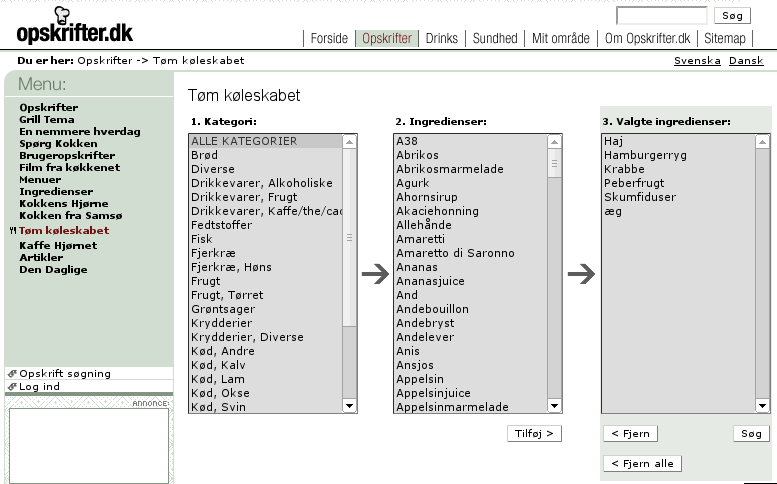
\includegraphics[scale=0.6]{billeder/forbilleder/opskrifterdk.png}
\capt{Brugergrænsefladen for Opskrifter.dk’s ``Tøm køleskabet''-funktion.}
\label{fig:opskrifterdk1}
\end{figure}

Søgningen foretages blandt de ca. 2700 opskrifter, som er tilgængelige på Opskrifter.dk. Resultaterne vælges ud fra, om de inkluderer minimum én af de valgte ingredienser. Under hver opskriftnavn vises antallet af valgte ingredienser, som opskriften inkluderer, men det er umiddelbart ikke muligt at sortere resultaterne efter dette tal. Klikker man på et resultat, åbnes den valgte opskrift til højre for resultaterne, og altså ikke på en ny side eller i et nyt vindue/faneblad. Opskrifterne viser informationer såsom tilberedningstid samt alle ingredienserne og deres mængder. Det er på alle opskrifter muligt at skalere opskriften til et bestemt antal personer. Figur \ref{fig:opskrifterdk2} viser et eksempel af et søgningsresultat. 

Kvaliteten af opskrifterne er forholdsvis høj og ca. 40 \% af alle opskrifter er med billede. Dette skyldes sandsynligvis, at det ikke er muligt for almindelige brugere direkte at indsende opskrifter. Almindelige brugere kan derimod indsende opskriftforslag, som først skal gennemlæses og tilføjes af en administrator.

\begin{figure}
\centering
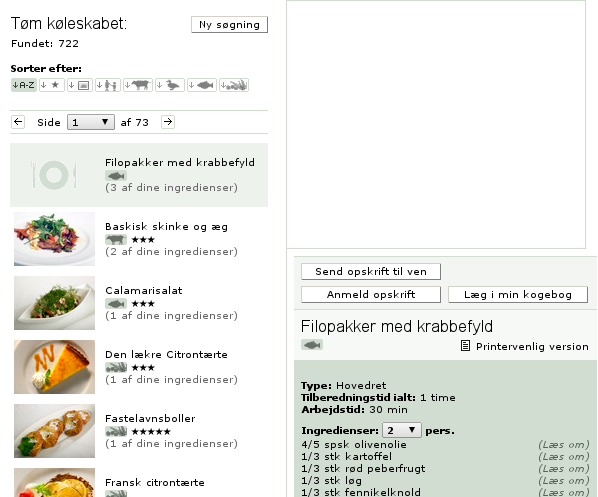
\includegraphics[scale=0.7]{billeder/forbilleder/opskrifterdk2.png}
\capt{Resultatsiden vist ved søgning med Opskrifter.dk’s ``Tøm køleskabet''-funktion. Her er markeret en opskrift, der ikke indeholder et billede af retten.}
\label{fig:opskrifterdk2}
\end{figure}

Opskrifter.dk har også et brugersystem, der tillader brugere at registrere sig og logge ind. Dette giver mulighed for, at man bl.a. kan gemme de opskrifter, man har fundet (ved at klikke på ``Læg i min kogebog''). Derudover husker ``Tøm køleskabet''-funktionen de ingredienser, man har indtastet, til næste gang man besøger siden.
Under ``Tøm køleskabet''-funktionen er det også muligt for brugeren at skrive kommentarer til funktionen. Disse kommentarer har givet et indblik i, hvad Opskrifter.dk’s brugere synes om funktionaliteten. Nogle kommentarer går på manglende ingredienser, mens en stor del kommentarer går på, at funktionen finder opskrifter, som man ikke kan lave uden at skulle købe en masse ind. \Fx skriver brugeren Jytte Hasselriis:

%kilde: http://opskrifter.dk/Toem-koeleskabet.149.0.html
\begin{quote}
``Hvordan skulle jeg kunne lave fasan i flødesovs, når jeg ikke har en fasan i køleskabet????'' \cite{opskrift-fasan}
\end{quote}

Dette synes at udtrykke en vis utilfredshed med den måde, hvorpå Opskrifter.dk’s ``Tøm køleskabet''-funktion vælger resultater på.